\chapter{Data and Methodology}
\label{chap:met}

\section{Data}

	\subsection{Universe of Stocks}
		The dataset, sourced at Reuters Datastream, comprises of liquid publicly traded shares from developed countries of Europe, Japan and Asia-Pacific (Australia, New Zealand, Hong Kong, and Singapore). The data is monthly and spans from 1990 to 2018. It comprises 8,350 companies, totaling 1,607,117 observations. An average firms is present for 16 years (192 observations). The data are rather evenly distributed in time, with 4,618 observations (firms) in an average month. 
		
		It is advantageous that the universe of these stocks is highly liquid, because it means that the firms are easily tradable with high volume and low transaction costs. This makes the results of this thesis more realistic (in terms of profitability of the trading strategy) and relevant (in terms of model interpretability), as the findings are not likely to be driven by illiquidity issues. The liquidity filter is obtained from \cite{tobek2020does}.  
	
	\subsection{Predictors as Distillation of Prior Literature}
		Table \ref{tab:meta} shows all 30 return predictors studied in this thesis. According to \cite{tobek2020does}, these variables are the best predictors of equity returns out of 153  candidate variables from leading financial and accounting journals (Figure 8 in \cite{tobek2020does}, global liquid universe of stocks). For each variable, Table \ref{tab:meta} gives the bibliographic reference to the original paper that proposed it as equity return predictor, as well as the publishing journal. Column Category presents the categorization of the features by the underlying data based on which the variable is calculated. Column Subcategory further discriminates the features based on the broad economic motivation for the feature as a return predictor. Finally, column Frequency shows the frequency (yearly or monthly) with which the feature changes values (is updated as new underlying data becomes available). [TODO make citations work, better classify the features into subcategories].   
	 
		\begin{table}
			\resizebox{\textwidth}{!}{\begin{tabular}{llllll}
\toprule
{} &        Data Source &               Category &                             Author & Journal & Frequency \\
Feature                                    &                    &                        &                                    &         &           \\
\midrule
52-Week High                               &             Market &             Behavioral &                \cite{george200452} &      JF &         M \\
Short-Term Reversal                        &             Market &             Behavioral &       \cite{jegadeesh1990evidence} &      JF &         M \\
Idiosyncratic Risk                         &             Market &       Attitude to risk &                \cite{ang2006cross} &      JF &         M \\
Volume / Market Value of Equity            &             Market &            Illiquidity &       \cite{haugen1996commonality} &     JFE &         M \\
Coefficient of Variation of Share Turnover &             Market &       Illiquidity Risk &          \cite{chordia2001trading} &     JFE &         M \\
Maximum Return                             &             Market &       Attitude to risk &              \cite{bali2011maxing} &      JF &         M \\
Whited-Wu Index                            &         Accounting &  Financial Constraints &         \cite{whited2006financial} &     RFS &         M \\
Coskewness                                 &             Market &       Attitude to risk &       \cite{harvey2000conditional} &      JF &         M \\
Operating Profits to Assets                &         Accounting &      Limited attention &            \cite{ball2016accruals} &     JFE &         Y \\
Lagged Momentum                            &             Market &             Behavioral &            \cite{novy2012momentum} &     JFE &         M \\
Liquidity Beta 5                           &             Market &       Illiquidity Risk &            \cite{acharya2005asset} &     JFE &         M \\
RD / Market Equity                         &         Accounting &      Limited attention &               \cite{chan2001stock} &      JF &         Y \\
Seasonality 6-10 A                         &             Market &            Seasonality &       \cite{heston2008seasonality} &     JFE &         M \\
Seasonality 11-15 N                        &             Market &            Seasonality &       \cite{heston2008seasonality} &     JFE &         M \\
Seasonality 2-5 N                          &             Market &            Seasonality &       \cite{heston2008seasonality} &     JFE &         M \\
Momentum-Reversal                          &             Market &             Behavioral &        \cite{jegadeesh1993returns} &      JF &         M \\
Amihud's Measure (Illiquidity)             &             Market &            Illiquidity &       \cite{amihud2002illiquidity} &     JFM &         M \\
Net Operating Assets                       &         Accounting &      Limited attention &    \cite{hirshleifer2004investors} &     JAE &         M \\
Seasonality 6-10 N                         &             Market &            Seasonality &       \cite{heston2008seasonality} &     JFE &         M \\
Seasonality                                &             Market &            Seasonality &       \cite{heston2008seasonality} &     JFE &         M \\
Seasonality 2-5 A                          &             Market &            Seasonality &       \cite{heston2008seasonality} &     JFE &         M \\
Accruals                                   &         Accounting &      Limited attention &             \cite{sloan1996create} &      AR &         Y \\
Duration of Equity                         &         Accounting &           Value effect &           \cite{dechow2004implied} &     RAS &         Y \\
Change in Common Equity                    &         Accounting &      Limited attention &  \cite{richardson2006implications} &      AR &         Y \\
Profit Margin                              &         Accounting &      Limited attention &              \cite{soliman2008use} &      AR &         Y \\
Liquidity Beta 3                           &             Market &       Illiquidity Risk &            \cite{acharya2005asset} &     JFE &         M \\
Liquidity Shocks                           &             Market &            Illiquidity &           \cite{bali2013liquidity} &     RFS &         M \\
Leverage Component of Book/Price           &         Accounting &           Value effect &              \cite{penman2007book} &     JAR &         Y \\
Earnings Predictability                    &         Accounting &       Attitude to risk &            \cite{francis2004costs} &      AR &         Y \\
Earnings Forecast-to-Price                 &  Analyst Forecasts &      Limited attention &           \cite{elgers2001delayed} &      AR &         M \\
\bottomrule
\end{tabular}
}
			\caption{Categorization of the Features}
			\label{tab:meta}
		\end{table}
	
	\subsection{Data Cleaning}
	
		Before feeding the data to the neural network, it is crucial to suitably clean them so that they are as informative as possible. As neural networks work best when the values of all features are on the same scale, the data are centered (by subtracting the mean) and then normalized so that all features range between the values $-1$ and $1$, as in \cite{gu2020empirical}. However, this operation would be highly problematic in the presence of outliers: if a feature has observations several times as high (or as small) as the rest of the data, normalization between $-1$ and $1$ would set the outliers' values close to $1$ (or $-1$), while setting the remaining majority of the values close to 0, thus rendering the data completely uninformative. To avoid this, the outliers are treated before normalization.
		
		The correct treatment of the outliers depends on whether the outlier value is a valid observation or not. In the former case, we should keep the observation, but clip the value so that it does not disturb the normalization, while in the latter case we should treat the value as missing, since it is likely due to errors in the data. Of course, the two cases are impossible to tell from each other from certainty, so the approach here is to declare values outside 2 standard deviations from the mean as erroneous and treat them as missing, and subsequently winsorize the data at 1\% bottom and 5\% top. Winsorization preserves the observation being treated, but clips it to the value of the corresponding percentile (1\% and 95\%). This approach to treating outliers was selected by inspecting the histograms of all variables with the aim that the normalization preserves the data distribution as well as possible.    
		
		Lastly, since all data fed to the neural network must be real numbers, missing observations must be imputed. Here, the missing data are replaced by 0, which is suitable, since the normalization between $-1$ and $1$ allows to interpret the value of $0$ as "no signal". The predictors vary considerably as to the percentage of missing data, as documented in Figure \ref{fig:missing_observations}. This is important, as the predictors with many missing values are likely to be less informative, as they offer less space for learning. The variables calculated directly from past returns, such as 52-Week High, Short-Term Reversal, Idiosyncratic Risk and Maximum, have almost no missing values. On the other hand, the ratio of research and development expenses to market value (RD / Market Equity) has more than 60\% of values missing, as some firms do not report research and development in their accounts. Other variables with many missing values are Earnings Predictability and Earnings Forecast-to-Price (around 50\% and 40\%). These are calculated based on analysts' forecasts, that are sometimes unavailable. The rest of variables have typically between 5\% and 20\% of missing values.  
		
		\begin{center}
			\begin{figure}
				\includegraphics[width=\textwidth,height=\textheight,keepaspectratio]{Figures/missing_observations.pdf}
				\caption{Amount of Missing Values in Individual Features}
				\label{fig:missing_observations}
			\end{figure}
		\end{center}
		
		These data-cleaning operations must be employed in a suitable order, which is: masking most extreme outliers as missing, imputing missing values by $0$, winsorizing, centering and normalizing. Of course, all the transformations are performed feature-wise, that is, always considering a single feature at a time. Less obviously, the transformations are performed on data grouped by years, that is, first splitting the data into groups by year, then applying the transformations and finally combining back into single dataset. The main motivation for this is to prevent information from spilling between training, validation and test sets, which are also organized by years.  
	
	\subsection{Predictor Descriptives}   	
	
		This subsection describes basic statistical properties of individual predictors (features) after cleaning, which is precisely the data entering the neural network. (The terms \textit{predictors}, \textit{variables} and \textit{features} are used interchangeably.) 
		 
		Since all the features are normalized to have 0 mean and to fit into the interval $-1$ and $1$, possibly the most important statistic to describe their distribution is standard deviation, plotted in Figure \ref{fig:standard_deviation}. It typically ranges between 0.2 and 0.5, with most features having standard deviation around 0.35. This is relatively high, meaning that the values are well-distributed in their $[-1,1]$ interval. Having high enough standard deviation is an important aspect of an informative feature: since the values are very different across observations, there is room for the model to learn from these differences. Three features have standard deviation below 0.2: Liquidity Shocks, Leverage Component of Book/Price and Profit Margin. On the other hand, three features have notably high standard deviations (above 0.5): Whited-Wu Index, Liquidity Beta 5 and Net Operating Assets. 
		
		\begin{center}
			\begin{figure}
				\includegraphics[width=\textwidth,height=\textheight,keepaspectratio]{Figures/standard_deviation.pdf}
				\caption{Standard Deviation of the Features}
				\label{fig:standard_deviation}
			\end{figure}
		\end{center}
		
		Other aspects of the unconditional features distributions are shown in the Appendix \ref{chap:additional_figures}. Specifically, Table \ref{tab:descriptives} gives mean, minimum, maximum, and 25th, 50th and 75th percentile of all features. The distributions are also summarized visually using histograms in Figure \ref{fig:histograms}.  
	
			
		Figure \ref{fig:correlation_matrix} shows the correlations of all features. The correlation matrix is also presented in a table form in the Appendix \ref{chap:additional_figures}.
		
		\begin{center}
			\begin{figure}
				\includegraphics[width=\textwidth,height=\textheight,keepaspectratio]{Figures/correlation_matrix.pdf}
				\caption{Features Correlation Matrix}
				\label{fig:correlation_matrix}
			\end{figure}
		\end{center}
		
		 Figure \ref{fig:correlation_matrix_highest} shows a smaller part of this matrix, subset so that the 10 most correlated feature pairs are shown. The correlation coefficients of these pairs are listed in Table \ref{tab:most_correlated_pairs}.
		 
		% Correlation matrix and table showing 10 most correlated pairs
		\afterpage{%    % defer execution until the next page break occurs anyway
			\begin{center}
				\begin{figure}
					\includegraphics[width=\textwidth,height=\textheight,keepaspectratio]{Figures/correlation_matrix_highest.pdf}
					\caption{Features Correlation Matrix (Subset to Show 10 Most Correlated Pairs)}
					\label{fig:correlation_matrix_highest}
				\end{figure}
			\end{center}
			
			\begin{table}
				\resizebox{\textwidth}{!}{\begin{tabular}{llr}
\toprule
                        &                      &  Correlation Coefficient \\
\midrule
Idiosyncratic Risk & Maximum Return &                    0.817 \\
Seasonality & Seasonality 2-5 A &                    0.555 \\
Liquidity Beta 5 & Liquidity Beta 3 &                   -0.512 \\
Amihud's Measure (Illiquidity) & Liquidity Shocks &                   -0.494 \\
Coefficient of Variation of Share Turnover & Amihud's Measure (Illiquidity) &                    0.405 \\
Seasonality & Seasonality 6-10 A &                    0.403 \\
Short-Term Reversal & 52-Week High &                    0.382 \\
Momentum-Reversal & Seasonality 2-5 N &                    0.370 \\
Duration of Equity & Leverage Component of Book/Price &                   -0.367 \\
Change in Common Equity & Net Operating Assets &                    0.353 \\
\bottomrule
\end{tabular}
}
				\caption{10 Most Correlated Pairs of Features}
				\label{tab:most_correlated_pairs}
			\end{table}
		} % end of argument of `\afterpage` command
		
		
		
	\subsection{Descriptives of Predicted Variable}
		The predicted variable is the return of stock $i$ in month $t$. The prediction is based on the predictors as available at the end of the previous month. (Borrowing from ML terminology, this thesis also uses the term \textit{target} to refer to the predicted variable.) 
		
		Figure \ref{fig:hist_returns} shows histogram of monthly returns. 
			
		\begin{center}
			\begin{figure}
				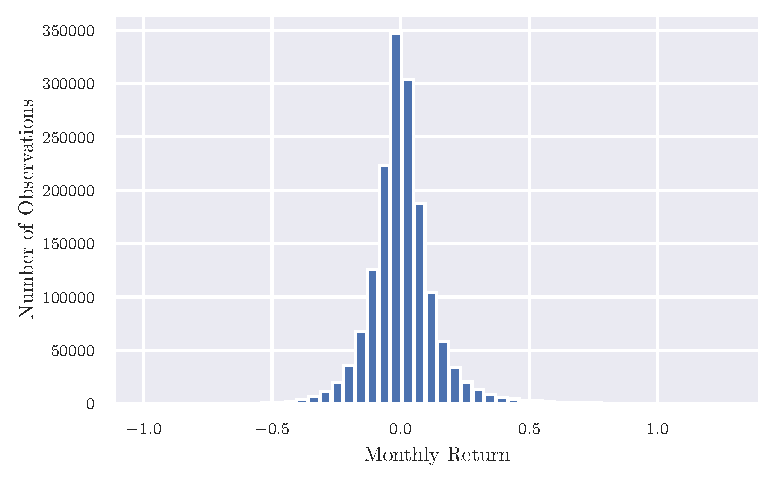
\includegraphics{Figures/hist_returns.pdf}
				\caption{Histogram of Monthly Returns}
				\label{fig:hist_returns}
			\end{figure}
		\end{center}


\section{Methodology}

	I train 5 distinct feed-forward neural networks, each with 9 different random seeds. The architecture and training follows closely \cite{gu2020empirical}, which represents very standard neural networks used in the task of equity return prediction from anomaly data. I compare the performance to that reached in the very same paper. Next, I interpret the neural networks using feature importance and investigate whether this interpretability is robust across different random seeds. I also investigate whether the interpretation of the model is stable in time. This  section describes the methodological issues related, in this order, to the model's architecture, training, performance evaluation and interpretation of the neural networks employed in this thesis.
	
	\subsection{Architecture of the Neural Networks}
	
	The prediction task is a regression of a stocks' returns in the following month on a set of the stocks' charasteristics calculated as of the current month. My neural networks' architecture follows closely \cite{gu2020empirical}, which studies the very same prediction task. In brief summary: all networks are feed-forward with the input dimension 30 and the output dimension 1; models of 5 different depths are used, with 1, 2, 3, 4, and 5 hidden layers consisting of 32, 16, 8, 4, and 2 neurons each respectively; all layers are fully connected, with batch-normalization \citep{ioffe2015batch} and ReLU activations on all hidden layers. As this is a regression problem, there is no activation on the output layer. The weights are regularized using L1 penalty. The following explains and motivates these choices in detail.
	
	First, let us describe a feed-forward neural network in general terms (e.g., \cite{goodfellow2016deep}). A feed-forward neural network can be represented as directed graph, consisting of several \textit{layers}. The input layer consists of several \textit{neurons} (nodes in the graph). This layer is connected to the next layer of neurons (the first hidden layer) by edges going from each input neuron to each hidden layer neuron. When each neuron of a layer is connected to each neuron in the next layer, we say that the two layers are fully connected. Each edge connecting two neurons is parametrized by a single trainable weight. More hidden layers can be connected to the previous hidden layer in the same fashion. Finally, the last hidden layer is connected, again, fully, to the output layer, which is the final prediction.
	
	This directed graph is a representation of the computation performed by the neural network to get from the input to the output. The values of a given hidden layer, \vec{h}, are computed using the previous layer's values $\vec{x}$, and the matrix of weights on the edges $\vec{W}$ using sum of products: 
	
	\begin{equation}
		\vec{h} = f(\vec{W}\vec{x})
	\end{equation}
	
	or written element-wise, the value of neuron $h_i$ in the hidden layer is computed as 
	
	\begin{equation}
		h_i = f \left( \sum_{j}w_{i,j}x_j \right)
	\end{equation}
	
	where the function $f$ is a non-linear activation function, such as the rectified linear unit (ReLU):
	
	\[
		f(z) = \text{ReLU}(z) =   
			\begin{cases}
				1 & \text{if } z \geq 0\\
				0 & \text{otherwise}
			\end{cases}.
	\]
	
	The output layer is computed using the last hidden layer in the same manner, except there is no activation function (in case of a regression problem at least). That is, denoting $\vec{V}$ the weights on the last edges and $\vec{h}$ the output of the last hidden layer, the output of the neural network $\vec{o}$ has the elements: 
	
	\begin{equation}
		o_i = \sum_{j}v_{i,j} h_j.
	\end{equation}
	
	In this thesis, the output is a scalar, so this further simplifies to 
	
	\begin{equation}
		o = \sum_{j}v_{j} h_j.
	\end{equation}
	
	In the case of neural network without hidden layers, the model simplifies to linear regression. Adding a hidden layer, which is a non-linear interaction of the previous layer's neurons, the input features are allowed to interact in any manner. Essentially, a hidden layer represents the input features in a sparser manner, generating more abstract information from them. This information then enters the next hidden layer and the information is made yet more concentrated. This continues until the output layer, which produces the most high-level information: the prediction. In this way, the network learns to find relationships between the features such that they predict the target (here, the return) well. The network's depth corresponds to the complexity of the model: the model with a single hidden layer can be considered the least complex one, as the inputs only enter one non-linear interaction, and the complexity increases up to 5 hidden layers, where the most abstract or high-level information is extracted.
	
	In this thesis, a neural network takes input of 30 real numbers (the stock's characteristics at given time point, dimension of the input layer) and propagates it through the series of hidden layers to produce the return prediction.	A choice must be made as to the number of hidden layers and number of neurons in each layer. While on optimal architecture can be searched for, here it is not necessary, as reaching the best possible performance is not the goal of this thesis. Instead, I follow \cite{gu2020empirical} and use the same numbers of layers and neurons as they, adapted to reflect my smaller size of input layer. I train models of 4 different depths: 1, 2, 3, and 4 hidden layers. The first hidden layer comprises of 16 neurons. Subsequent layers, if used, contains 8, 4 and 2 neurons for the second, third and fourth layer respectively. Note that the decreasing number of neurons is why we say the information is becoming more and more concentrated the deeper the hidden layer. Throughout the thesis, these 4 distinct neural networks are referred to as NN1, NN2, NN3 and NN4, the number standing for the respective number of hidden layers in the network.
	
	One of the neural networks used in this thesis, particularly, NN2 (the network with two hidden layers), is visualized here: 
	
	\tikzset{%
		every neuron/.style={
			circle,
			draw,
			minimum size=1cm
		},
		neuron missing/.style={
			draw=none, 
			scale=4,
			text height=0.333cm,
			execute at begin node=\color{black}$\vdots$
		},
	}
	
	\begin{center}
		\begin{figure}
			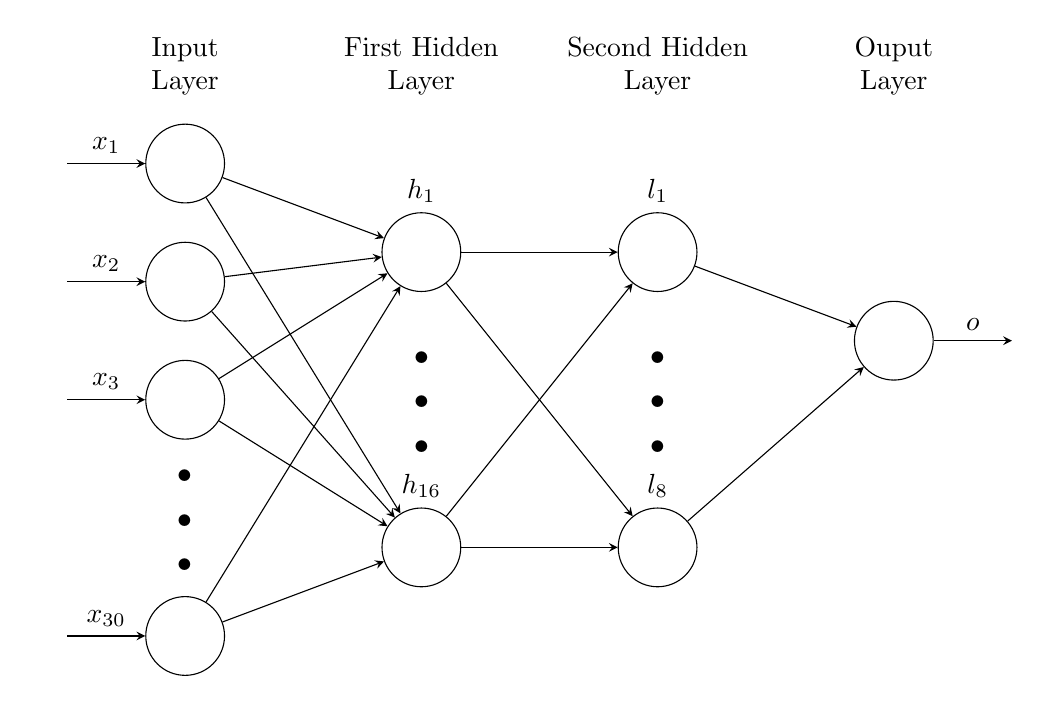
\begin{tikzpicture}[x=1.5cm, y=1.5cm, >=stealth]
			% draw nodes in input layer
			\foreach \m/\l [count=\y] in {1,2,3,missing,4}
			\node [every neuron/.try, neuron \m/.try] (input-\m) at (0,2.5-\y) {};
			
			% draw nodes in hidden layers
			\foreach \m [count=\y] in {1,missing,2}
			\node [every neuron/.try, neuron \m/.try ] (hidden1-\m) at (2,2-\y*1.25) {};
			
			% draw nodes in hidden layers
			\foreach \m [count=\y] in {1,missing,2}
			\node [every neuron/.try, neuron \m/.try ] (hidden2-\m) at (4,2-\y*1.25) {};
			
			% draw nodes in output layer
			\foreach \m [count=\y] in {1}
			\node [every neuron/.try, neuron \m/.try ] (output-\m) at (6,0) {};
			
			% Annotate input neurons, draw input arrows
			\foreach \l [count=\i] in {1,2,3,30}
			\draw [<-] (input-\i) -- ++(-1,0)
			node [above, midway] {$x_{\l}$};
			
			% Annotate hidden neurons
			\foreach \l [count=\i] in {1,16}
			\node [above] at (hidden1-\i.north) {$h_{\l}$};
			
			% Annotate hidden neurons
			\foreach \l [count=\i] in {1,8}
			\node [above] at (hidden2-\i.north) {$l_{\l}$};
			
			% Annotate output neurons, draw output arrows
			\foreach \l [count=\i] in {1}
			\draw [->] (output-\i) -- ++(1,0)
			node [above, midway] {$o$};
			
			% Draw arrows between input and hidden
			\foreach \i in {1,...,4}
			\foreach \j in {1,...,2}
			\draw [->] (input-\i) -- (hidden1-\j);
			
			% Draw arrows between hidden and hidden
			\foreach \i in {1,...,2}
			\foreach \j in {1,...,2}
			\draw [->] (hidden1-\i) -- (hidden2-\j);
			
			% Draw arrows between hidden and output
			\foreach \i in {1,...,2}
			\foreach \j in {1}
			\draw [->] (hidden2-\i) -- (output-\j);
			
			% Annotate layers
			\foreach \l [count=\x from 0] in {Input, First Hidden , Second Hidden, Ouput}
			\node [align=center, above] at (\x*2,2) {\l \\ Layer};
			\end{tikzpicture}
			\caption{Computation Graph of the Neural Network NN2}
			\label{fig:computation_graph}
		\end{figure}
	\end{center}
	
	In addition, I add a batch-normalization layer \citep{ioffe2015batch} after every hidden layer, again in line with  \cite{gu2020empirical}. This changes the above formula for hidden layer values to: 
	
	\begin{equation}
		\vec{h} = \text{ReLU}(\text{BN}(\vec{W}\vec{x}))
	\end{equation}
	
	where $\text{BN}$ represents the batch-normalization operation. The operation simply normalizes its input data (subtracts sample mean and divides by sample variance). The data is split to batches to improve computing speed of the operation. The operation helps with multiple aspects of training the neural networks, as it prevents the values coming out of a hidden layer from being extreme. This helps to regularize the network and also speeds up the training. Importantly, it helps with the problem of "internal covariate shift", where the distributions of inputs to hidden layers are shifted relative to their validation and testing counterparts, which harms the predictive power and the convergence. By demeaning and standardizing the data, batch normalization preserves the information contained in the hidden layer while preventing the covariate shift \citep{ioffe2015batch}. 
	
	
	\subsection{Training, Regularization and Hyperparameter Tuning}
	
	In general terms, training any neural network amounts to searching for such weights on its edges such that the loss on the training data (typically reflecting the prediction error) is small. The optimization is done numerically, by iteratively adjusting the weights so that a loss is gradually decreasing. At the beginning of training, the model is initialized with small random weights, where the random state is determined using the so-called random seed. Prediction is computed using these weights, which are then adjusted using the negative gradient of the loss. This is applied iteratively until a stopping criterion is met and the final weights are extracted. This thesis uses mean squared error as the loss, as the prediction task is a regression.
	
	The data is fed to the network in so-called batches, meaning that several inputs are processed together and the weight update is calculated across the whole batch. When all training data-points have been fed to the network exactly once, we say one epoch has passed. This is repeated for a number of epochs. I use batch size of 5,000, which is enough for processing the data reasonably fast while not overflowing the memory. I use 100 epochs in line with \cite{gu2020empirical}, but this number is never actually reached during the training (it works just as an upper limit), due to early stopping, as explained below.
	
	There are several optimizers one can use to descend the slopes of the loss function. In line with \cite{gu2020empirical}, I use Adam optimizer. The advantage of Adam is two-fold. First, it essentially lowers the learning rate as the training progresses. The learning rate governs how much the weights are adjusted in a given direction (in the direction of negative gradient of the loss in the simple case of Stochastic Gradient Descent optimizer). Shrinking the learning rate gradually allows faster learning at the beginning of the training and a more nuanced convergence near the optimum [TODO add citation]. [TODO refresh the theory behind using Adam and describe the advantages better]. (In about 1\% of the cases, the optimized model learns to predict just the average of the training data. I retrain these models using Stochastic Gradient Descent optimizer with Nesterov momentum 0.99.)
	
	Neural networks are non-parametric way of modeling the relationship between the predictors and the predicted variables, in the sense that there is no a priori assumption made about the functional form of the relationship. In fact, the Universal Approximation Theorem shows that with already a single hidden layer, the network outlined above is able to approximate any "well-behaved" function arbitrarily well. This is directly opposed to the linear approach, where we fit the relationship between inputs and outputs assuming a linear functional form. 
	
	This necessarily means that neural networks are prone to overfitting the training data. An overfitted model performs well on the training data and poorly on previously unseen data. This is a problem, as the point of having a model in the first place is to be able to draw general conclusions and predict from new data. This is why the models are evaluated solely on held-out data (testing sample), which is disjoint from both training and validation sample, both for purposes of measuring performance and interpreting the models. In addition, there is a number of methods that can be used to prevent overfitting on the training data in the first place, commonly called regularization. The goal is to limit the training process to prevent overfitting while leaving enough room for learning. I use the same regularization techniques as \cite{gu2020empirical}, namely, learning rate shrinkage, batch normalization, early stopping, weight regularization, and ensembling. I have already discussed the use of batch normalization and learning rate shrinkage. I now describe how I use the remaining methods. 
	
	Early stopping amounts to ceasing the training at some earlier point than reaching the pre-specified number of epochs. To determine that point, one can evaluate the model's predictive power after each epoch. A subsample of the data disjoint from training data (called validation sample) is used for the evaluation. This simulates the out-of-sample performance. When the validation loss increases for $k$ consecutive epochs ($k$ is called patience), training is stopped. In line with \cite{gu2020empirical}, I use patience of 5. 
	
	Weight regularization allows to punish the model for finding too big weights, as large weights are a symptom of overfitting. The size of weights can be measured as their L2 or L1 norm, L1 norm is used here. The strength of the weight regularization is chosen as a hyperparameter on validation data and line with \cite{gu2020empirical}, as described below in the section on hyperparameter tuning.
	
	Ensembling, averaging the predictions of multiple models, is widely discussed in the Literature Review. It can be considered a regularization technique, as different models can overfit to training data differently, their average takes out this error and thus is able to generalize better. I construct the ensembles in a common way and in line with \cite{gu2020empirical}, by averaging the same model across its different random seeds. I use 9 random seeds for each model (that is, for each train-validation-test split and each architecture). As models with different random seed can be trained in parallel, this does not place a burden on the computation time.
		
	The remaining modeling choices (starting learning rate and strength of L1 regularization) are done using hyperparameter tuning. The hyperparameters discussed so far are not very data-specific, so it suffices to choose them using prior literature: I use \cite{gu2020empirical}, as we share the exact same prediction task. However, there are parameters that are very data-specific, and must therefore be chosen using the data. Choosing the parameters on the training data would lead to overfitting, which is why they are selected using a sample disjoint from training data, called validation sample. This is called hyperparameter tuning. Specifically, I tune the learning rate and the strength of L1 regularization. Each model (each of its 9 random seeds) is run 20 independent times, each time sampling the learning rate and the L1 hyperparameters randomly from pre-specified intervals using logarithmic distribution. The intervals are $\left[1\mathrm{e}{-3}, 1\mathrm{e}{-2}\right]$ and $\left[1\mathrm{e}{-5}, 1\mathrm{e}{-3}\right]$ respectively, again in line with \cite{gu2020empirical}. A single best instance is then selected, as determined by predictive performance of the model on the validation set.
	
	The train-validation-test split is done as follows. There are 29 years of data in the entire dataset, with rather evenly distributed observations from 1990 to 2018. The first 12 years of data are used as training set. The next 12 years are used as the validation set, and the year after that as the test set. To investigate how the model changes in time, more splits are performed: each year, the training data is rolled forward using expanding window (that is, taking 13 years from the beginning of the dataset, 14, 15 etc.). Validation set is rolled forward using fixed window (always consisting of 12 years) and starts directly at the end of the corresponding training set, and the test set is rolled forward also using fixed window (always consisting of 1 year) and starts directly at the end of the corresponding validation set. The train-validation-test split can be therefore summarized as 12-12-1, 13-12-1, 14-12-1, 15-12-1 and 16-12-1, where the last split uses all 29 years in the dataset. Each time a different split is taken, the model is retrained from scratch. This approach reflects that of \cite{gu2020empirical}, adjusted appropriately to my shorter dataset (29 years instead of 60) and is used instead of cross-validation so that the temporal ordering of the data is preserved (the model is trained on the past and evaluated on the future, never in the reverse).    


	\subsection{Performance Evaluation}
	The predictive performance of the models is measured using several metrics – $R^2$, root-mean-squared error (RMSE) and mean-absolute error (MAE). As all the models are evaluated on the test set, whose data were never used during training and hyperparameter tuning, we call all these metrics out-of-sample (OOS), as opposed to in-sample. It is important to use the out-of-sample metrics to be sure that the results are not due to overfitting. 
	
	$R^2$ is here defined slightly differently than usual:
	
	\begin{equation}
		R^2_{OOS} = 1 - \frac{ \sum_{(i,t)\in T_3} \left(r_{i,t+1}-	\hat{r}_{i, t+1}\right) ^2}{\sum_{(i,t)\in T_3} r_{i,t+1}^2}, 		
	\end{equation}
	
	where $T_3$ indicates the testing sample. This is also the definition of $R^2$ used by \cite{gu2020empirical}. As the usual $R^2$, it measures how much of the variance in the predicted variable (here, return) is explained by the model, but it is distinct from the usual $R^2$ in that there is no demeaning in the denominator. This means that instead of comparing the forecasts to the naive forecast of average return, the metric compares predictions to the naive forecast of zero returns. This is because in the task of predicting individual stock returns, forecasts using global average often underperfom those using just zero, so using the usual $R^2$ definition would be too low a hurdle \citep{gu2020empirical}. 
	
	The RMSE is defined in the usual manner:   
	
	\begin{equation}
		RMSE_{OOS} = \sqrt{ \frac{1}{|T_3|} \sum_{(i,t)\in T_3} \left(r_{i,t+1}-	\hat{r}_{i, t+1}\right) ^2},	
	\end{equation}
	
	and represents the average squared error of the prediction after taking a root of it, which is done so that the final measure is directly comparable in scale to the original returns. Note that it is very similar to the numerator of $R^2$.
	
	The MAE is defined as usual as well: 
	
	\begin{equation}
		MAE_{OOS} = \frac{1}{|T_3|} \sum_{(i,t)\in T_3} |r_{i,t+1}-	\hat{r}_{i, t+1}|
	\end{equation}
	
	and differs from RMSE just in taking absolute value of the error instead of square, which gives same weight to large errors as to the small ones, as opposed to RMSE where large errors have larger weights (rising with their square). 
	
	
	\subsection{Interpretation}
	
	Possibly the most straightforward way of interpreting any model is to show how individual predictors contribute to the prediction, in other words, which explanatory variables matter the most and which are less important. This notion is called \textit{feature importance} and can be generally thought of as the ML counterpart to the size of coefficients in a linear regression. Feature importance can be measured locally or globally. The former approach studies why a particular observation is assigned its prediction: how can the prediction be attributed to individual predictors? The latter explains how the model decides overall, across all observations. This thesis investigates two methods of feature importance, Model Reliance \citep{fisher2019all} (which is a global measure) and Integrated Gradients \citep{sundararajan2017axiomatic} (a local measure). In addition, Integrated Gradients are also used here as a global measure, by taking their average of absolute values across observations. The reasons behind choosing these measures as well as their theoretical underpinnings are explained in detail in the Literature Review. This section describes the technical aspects of the measures' calculation.
	
	\subsubsection{Model Reliance}
		Model Reliance \citep{fisher2019all} is a global measure of feature importance. It is based on the idea that if a feature is important for making prediction, then distorting the feature by adding noise to it will damage prediction performance. Vice versa, if distorting a feature leaves the prediction performance relatively intact, that feature can be considered unimportant for the prediction. Thus, denoting  the prediction function (such as an ML model) $f$, Model Reliance of  $f$ on random variable $X$ can be \textit{informally} defined as
		
		\begin{equation}
			MR(f):=\frac{\text{Expected loss of \textit{f} under noise}}{\text{Expected loss of \textit{f} without noise}},
		\end{equation}
		
		where the noise renders the random variable $X$ completely uninformative of the predicted variable while it at the same time does \textit{not} change the marginal distribution of $X$. More specifically, denote the predicted random variable as $Y$ and consider $X_1$ and $X_2$ as two explanatory random variables. The expected loss of $f$ can be then denoted as 
		
		\begin{equation}
			e_{\text{orig}}(f):= \mathbb{E} L(f,(Y,X_1, X_2)).
		\end{equation} 
		
		Further denote $X_1^s$ as random variable following the same marginal distribution as $X_1$, but independent of $Y$. 
		
		Then the expected loss of $f$ under noise, which distorts $X_1$ to $X_1^s$, can be denoted as 
		
		\begin{equation}
			e_{\text{switch}}(f):= \mathbb{E} L(f,(Y,X_1^s, X_2)).
		\end{equation} 
		
		Finally, Model Reliance can be \textit{formally} defined as 
		
		\begin{equation}
			MR(f):=\frac{e_{\text{switch}}(f)}{e_{\text{orig}}(f)}
		\end{equation}
		
		To see the intuition behind this formula, consider first the case that $X$ is very informative of $Y$. Then, 	$e_{\text{switch}}$ is much larger than $e_{\text{orig}}$ and Model Reliance is larger than 1. The more $X$ is informative of $Y$, the larger the  Model Reliance of $f$ on $X$ --- the more the model \textit{relies} on the feature to make the prediction. In the case when Model Reliance is exactly 1, the feature can be considered unimportant, as completely distorting it does not change the model's loss. Model Reliance can also be less than one, in the case that the distorted feature actually perform better than the original feature.
				
		The sample estimate of $e_{\text{orig}}(f)$ is the loss used in the model's training. Denote the target as $\vec{y} \in \mathbb{R}^N$ and consider two features $\vec{x_1}, \vec{x_2} \in \mathbb{R}^{N}$:
		
		\begin{equation}
			\hat{e}_{\text{orig}}(f):= \frac{1}{N} \sum_{i=1}^{N} L\left(f, (y_i, x_{1_i}, x_{2_i}) \right)
		\end{equation} 
		
		The sample estimate of $e_{\text{switch}}(f)$ can be done in two different ways, either by randomly permuting the values of the given feature or by dividing the feature's values in halves and the switching the halves. This thesis uses the latter, as it is computationally less demanding. (In both cases, the rest of the features and the predicted variables are intact.) It follows that the sample estimate of $e_{\text{switch}}(f)$ can be calculated as
		
		
		\begin{equation}
			\begin{split}
				\hat{e}_{\text{switch}}(f):= & \frac{1}{2 \lfloor N/2 \rfloor} \sum_{i=1}^{\lfloor N/2 \rfloor} L \left(f, \left( y_i, x_{1_{i+\lfloor N/2 \rfloor}}, x_{2_{i}} \right) \right) + \\ 
				& + L \left( f, \left(y_{i+\lfloor N/2 \rfloor}, x_{1_{i}}, x_{2_{i+\lfloor N/2 \rfloor}} \right) \right). 
			\end{split}
		\end{equation}
		
		This is simply the loss of the prediction using the same data as original, but with values in the feature $\vec{x_1}$ split in half and the halves swapped, leaving the other features (here, $\vec{x_2}$) and the predicted variable $y$ unchanged. (If $N$ is even, the split in half can be performed exactly, and if $N$ is odd, the last observation in the dataset is not used and the split is then performed in the same way as if $N$ is even.) The extension to the case with more than two features is straightforward: when calculating Model Reliance of feature $\vec{x_1}$, we disturbed the values in $\vec{x}_1$, leaving $\vec{y}$ and $\vec{x_2}$ unchanged. If we additionally have, say, $\vec{x_3}$ and $\vec{x_4}$, they are treated in the same way as $\vec{x_2}$, that is, unchanged. 
		
		Finally, the sample estimate of Model Reliance on a given feature is: 
		
		\begin{equation}
			\widehat{MR}(f):=\frac{\hat{e}_{\text{switch}}(f)}{\hat{e}_{\text{orig}}(f)}.
		\end{equation}
			
		That is, when calculating reliance of the model on a given feature, two predictions are made using the model: one is the usual one, with all features as well as the target undisturbed, the other is almost the same, except that we have disturbed the given feature (and the given feature only) by swapping halves of its values. The loss of both predictions is then computed as usual. Model Reliance is then the ratio of these two losses, the disturbed loss divided by the undisturbed one.   
		
		TODO: include algorithmic description as per \cite{molnar2020interpretable}.
	
		
	\subsubsection{Integrated Gradients}
		Integrated Gradients \citep{sundararajan2017axiomatic} is a local measure of feature importance, i.e., it is computed for each observation separately. It considers the gradient of the prediction with respect to the predictors. If a small change in a predictor's value has large effect on the prediction, the value of the gradient is large.
		
		Again, denote $f: \mathbb{R}^k \rightarrow \mathbb{R}$ the prediction function (here, the NN model). Further, denote $\vec{z} \in  \mathbb{R}^k$ a single input with $k$ scalar elements, where $k$ denotes the total number of features (here, 30). Let $\vec{z'} \in  \mathbb{R}^k$ be a \textit{baseline input}, an observation that can be considered as a point from which the other observations depart. (For example, in case of inputs being images, the baseline can be a black image. In this thesis, it is a vector of zeros, as motivated below.) 
		
		For simplicity of the notation, assume that $f: \mathbb{R}^k \rightarrow [0,1]$. The Integrated Gradient of $i^{th}$ feature of the input $\vec{z}$ is defined as 
		
		\begin{equation}
			IG_i(\vec{z}) := (z_i - z_i') \int_{\alpha=0}^{1} \frac{\partial f(\vec{z'} + \alpha(\vec{z}-\vec{z'}))}{\partial z_i}d\alpha,
		\end{equation}
		
		where $\frac{\partial f(\vec{z})}{\partial z_i}$ stands for the gradient of $f(\vec{z})$ along the $i^{th}$ dimension. This means that the measure considers a straight path in $\mathbb{R}^k$ from the baseline input ${\vec{z}'}$ to the given input ${\vec{z}}$ and calculates the gradient of prediction at all points along that path. The Integrated Gradient measure cumulates these gradients by taking the integral across the path.  
		
		To calculate the Integrated Gradient of $i^{th}$ feature of the input $\vec{z}$ empirically, it is necessary to approximate the integral by summation across several points along the straightline path  \citep{sundararajan2017axiomatic}. That is:  
		
		\begin{equation}
			IG_i^{\text{approx}}(\vec{z}) := (z_i - z_i') \sum_{k=1}^{m} \frac{\partial f(\vec{z'} + \frac{k}{m}(\vec{z}-\vec{z'}))}{\partial z_i}\frac{1}{m},
		\end{equation} 

		where $m$, called the \textit{step size}, is the number of the steps in the Reimman approximation of the integral, here, the number of points along the straightline path at which evaluate the gradient. 
		
		Two implementation decisions must be made when calculating the Integrated Gradients: first, choosing the right baseline input, and second, choosing the right the step size. First, the baseline input should be chosen such that it can be interpreted as "no signal". In this thesis, there are two possible baselines: random noise and all-zero input. The latter was chosen, as it lends itself well to the "no signal" interpretation: all the features are normalized between -1 and 1 and have a mean of 0, thus, an all-zero input can be considered a natural point of departure. Additionally, the authors recommend to check that the model's prediction at baseline is around zero. This is important because it allows to use Integrated Gradient to explain the prediction as a function of the input, and not as of the input and the baseline. Indeed, the predictions for the all-zero input are around zero, which confirms that the all-zero input is the correct baseline here. Second, the step size should be chosen such that the approximation is good enough: the authors recommend to check that the attributions approximately sum up to the difference between the prediction at $\vec{z}$ and at $\vec{z'}$. Given that the latter is around zero, it remains to check that the attributions for $\vec{z}$ sum up to the prediction at $\vec{z}$. (Note that this is a verification of passing the Completness Axiom, see Literature Review.) This thesis uses the step size of 50, which passes this summation check comfortably [TODO verify].  
		
		$\epsilon$, $\xi$